
\subsection{Results}

As an outcome from the effort on this work several results were obtained. This section will first talk about the synthesis configurations that were experimented and how each module is affected by them, following that the synthesis results are presented and finally the subset used for prototipation is explained.

\begin{table}[h]
\centering
\begin{tabular}{|l||c|c|c|c|c|c|}
\hline
  & \multicolumn{6}{|c|}{Synthesis Configurations} \\ \hline
  		& BASIC & PIPE  & MID   	& FST1  		& FST2  		& ASAP  \\ \hline
FrameControl 	&	& X	& X		& A$^*$  		& X			& S 	\\ \hline
DCT 		&       & X     & D$^*$	 	& U$^*$ F$^*$ D$^*$  	& D$^*$ U$^*$ F$^*$ P9  & S     \\ \hline
Quantizer	&       & X     & D$^*$	 	& U$^*$ F$^*$    	& D$^*$ U$^*$ F$^*$ 	& S     \\ \hline
VLC 		&       & P9    & X     	& U$^*$ F$^*$    	& D$^*$ U$^*$ F$^*$ A   $^*$& S P9   \\ \hline
Stream 		&       & X     & X		& A$^*$ $^D*$		& X			& S     \\ \hline
Match 		&       & X     & X      	& P9 A$^*$ D$^*$	& X			& S     \\ \hline
IQuantizer 	&       & P9    & D$^*$		& U$^*$ F$^*$    	& D$^*$ U$^*$ F$^*$  	& S     \\ \hline
IDCT 		&       & P9    & D$^*$		& U$^*$ F$^*$   	& D$^*$ U$^*$ F$^*$     & S     \\ \hline
IMotion 	&       & X     & D$^*$		& A$^*$ D$^*$ U		& X		        & S     \\ \hline
MV Coder 	&       & X     & X	 	& A$^*$ D$^*$ 		& X			& S     \\ \hline
Reference 	&       & X     & X     	& X      		& X      		& S     \\ \hline

\end{tabular}
\caption{Synthesis configurations used and it's options}
\label{tab:synthconfigs}
\end{table}

As explained earlier one of the great strengths of behavioral synthesis is the opportunity to explore the design space very quickly, without having to redesign the system architecture. In the MPEG encoder presented in this text different RTL implementation options have been generated for each module. 
This allows the best option to be picked according to the desired application requirements. Table \ref{tab:synthconfigs} enlists all the synthesis configurations used and what optimizations or transformations are applied to each module. The letters and symbols in the table body mean the following:
\begin{itemize}
\item U: loop unrolling is applied;
\item A: aggressive scheduling is applied;
\item F: array flattening is applied;
\item P\#: pipelining is applied with initiation interval \#;
\item L: latency from input to output is constraned a maximum amount of clock cycles;
\item D: data path optimization is applied;
\item S: all operations are scheduled as soon as possible and all global optimizations are on;
\item X: configurations marked with an X are not used on the corresponding module;
\item * modifier: the directive is applied globally on module.
\end{itemize}

After selecting the directives for each synthesis configuration each module was synthesized and simulated to check if the generated RTL worked. The synthesis results are presented in table \ref{tab:synthres}. The numbers in the data column labled with LE represents the number of logic elements used from the target FPGA, which in total contanis about 35000 logic elements, the number in parenthesis being the amount used for multiplexing. Next to it the column labled REG represents the count of register bits used by the module for that specific synthesis configuration and the LAT column representing the latency cycles (worst case) for each data block processed by the module (without accounting pipelining). Synthsis configurations that were not used in the modules are left in blank.

\begin{landscape}
\begin{table}[h]
\centering
\begin{tabular}{|l||c|c|c |c|c|c |c|c|c |c|c|c |c|c|c |c|c|c |}
\hline
 & \multicolumn{3}{|c|}{BASIC} &
   \multicolumn{3}{|c|}{PIPE} &
   \multicolumn{3}{|c|}{MID} &
   \multicolumn{3}{|c|}{FST1} &
   \multicolumn{3}{|c|}{FST2} &
   \multicolumn{3}{|c|}{ASAP} \\ \hline
%
 		& LUT  & REG & LAT & LUT  & REG & LAT & LUT  & REG & LAT & LUT  & REG & LAT & LUT  & REG & LAT & LUT  & REG & LAT \\ \hline
Frame		&1008 &979&2794k &  -   &  -  &  -  &  -   &  -  &  -  &1325  &763&1965k&   -  &  -  & -   &1608  &1862 &3209k\\ \hline
DCT		&1292  &1562 &1795 &13214 &8806 &33   &2070  &1322 &1795 &3849  &3348 &157  &12828 &7641 &38   &16998 &4963 &22   \\ \hline
Quant.		&1774  &935  &755  &  -   &  -  &  -  &1713  &931  &755  &2939  &2112 &83   &5927  &2399 &85   &7155  &3539 &40   \\ \hline
VLC		&3773  &5751 &844  &10051 &6753 &844  &  -   &  -  & -   &3210  &5743 &844  &3314  &2466 &845  &13412 &6899 &844  \\ \hline
Stream		&574   &198  &4    &  -   &  -  &  -  &  -   &  -  & -   &726   &305  &5    &  -   &  -  & -   &828   &232  &3    \\ \hline
Match		&3099  &2089 &6003 &  -   &  -  &  -  &  -   &  -  & -   &2674  &2358 &8817 &  -   &  -  & -   &4905  &3370 &6129 \\ \hline
IQuant.		&826   &477  &553  &  -   &  -  &  -  &528   &791  &553  &2774  &3333 &27   &2774  &3333 &27   &2848  &4334 &26   \\ \hline
IDCT		&1201  &1463 &2275 &  -   &  -  &  -  &2967  &1835 &247  &6222  &5738 &111  &6222  &5738 &111  &12373 &6664 &34   \\ \hline
IMotion		&1831  &607  &3980 &  -   &  -  &  -  &1311  &632  &2822 &1620  &1219 &5174 &  -   &  -  & -   &2871  &1048 &2054 \\ \hline
MV Code	 	&822   &305  &8    &  -   &  -  &  -  &  -   &  -  & -   &820   &477  &10   &  -   &  -  & -   &1523  &359  &5    \\ \hline
Refer.		&654   &470  &46   &  -   &  -  &  -  &  -   &  -  & -   &  -   &  -  &  -  &  -   &  -  & -   &895   &377  &39   \\ \hline
\end{tabular}
\caption{Resource usage for each module}
\label{tab:synthres}
\end{table}
\end{landscape}

After the synthesis of each module some simulations must be run to see which combination of configurations provide better performance so it can be picked to go through logic synthesis and placement and routing. Table \ref{tab:combination} shows the combibations of synthesis configurations that were pickes for the benchmarking while table \ref{tab:fps} shows the resulting frame rate for each of those combinations, remembering that 24 frames per second is the desired rate. For these tests only the modules used for the prototype (which generates only I-type frames) were used.

\begin{table}[h]
\centering
\begin{tabular}{|l||c|c|c|c|c|c|}
\hline
		& CFG1	& CFG2	& CFG3	& CFG4	& CFG5 & CFG6 \\ \hline
FrameControl 	& BASIC	& BASIC	& BASIC & FST1  & FST1 & ASAP \\ \hline
DCT		& BASIC & MID   & FST1  & FST1  & FST2 & ASAP \\ \hline
Quantizer	& BASIC & MID   & FST1  & FST1  & FST2 & ASAP \\ \hline
VLC		& BASIC & BASIC & FST1  & PIPE  & PIPE & ASAP \\ \hline
Stream		& BASIC & BASIC & BASIC & FST1  & FST1 & ASAP \\ \hline
\end{tabular}
\caption{Selected combinations of synthesis configurations}
\label{tab:combination}
\end{table}

\begin{table}[h]
\centering
\begin{tabular}{|l|c|c|}
\hline
Combination & Frame Rate & Total Area (LUT) \\ \hline
CFG1 & 1.1 & 8361\\ \hline
CFG2 & 2 & 9138\\ \hline
CFG3 & 7 & 11580\\ \hline
CFG4 & 26  & 18890 \\ \hline
CFG5 & 30  & 30917\\ \hline
CFG6 & 49  & 30001 \\ \hline
\end{tabular}
\caption{Framerate obtained for each combination of synthesis configurations }
\label{tab:fps}
\end{table}

With information from table \ref{tab:fps} it's possible to pick the design that fits the requirements using the minimum area. It's also possible to plot a graph that shows the results mapped into the design space, which is shown in figure \ref{fig:designspace}. The analysis of this data leads to pick the combinantion named CFG4 as the option to be prototyped beacause it's the configuration that beats 24fps taking the minimum area among the others. With further design space exploration and some fine-tuning it should to be possible to reduce area to less than 15000 LUTs while still beating 24fps performance.

\begin{figure}[h]
\centering
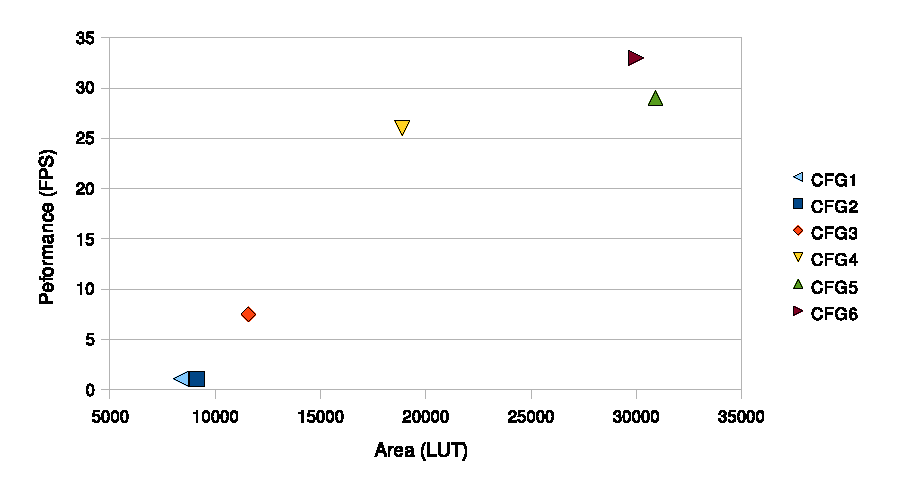
\includegraphics{figs/designspace.eps}
\caption{Graph of the explored design space}
\label{fig:designspace}
\end{figure}

